\section{Circuit Boards}
\label{sec:circuit_board}
After manufacture, Tiny Tapeout chips are mounted onto small carrier boards with 0.1~inch pin headers. These carriers allow people with limited surface mount technology (SMT) assembly experience to build their own demonstration boards around the chips.

The carrier fits onto the demonstration board shown in Fig.~\ref{fig:demonstration_board}. The demonstration board is designed primarily for ease of use by beginners, though offers enough flexibility for power users. As all signals are below \qty{50}{\MHz}, no special layout was needed in the design of the demonstration board.

The demonstration board provides:
\begin{itemize}
\item USB Type-C as a power connection,
\item \qty{1.8}{\V} and \qty{3.3}{\V} power supplies for core and IO,
\item \qty{20}{\MHz} oscillator,
\item Buttons for reset and single step clock,
\item An eight way DIP switch for inputs,
\item A nine way DIP switch for design selection,
\item A seven segment LED display for the outputs,
\item Headers for all IO, including two standard Digilent ports (PMOD),
\item A header to select the internal clock or to provide one externally,
\item A header to select an internal or external scan chain driver,
\item A header to engage an automatic clock divider in input pin zero.
\end{itemize}

\begin{figure}[!t]
\centering
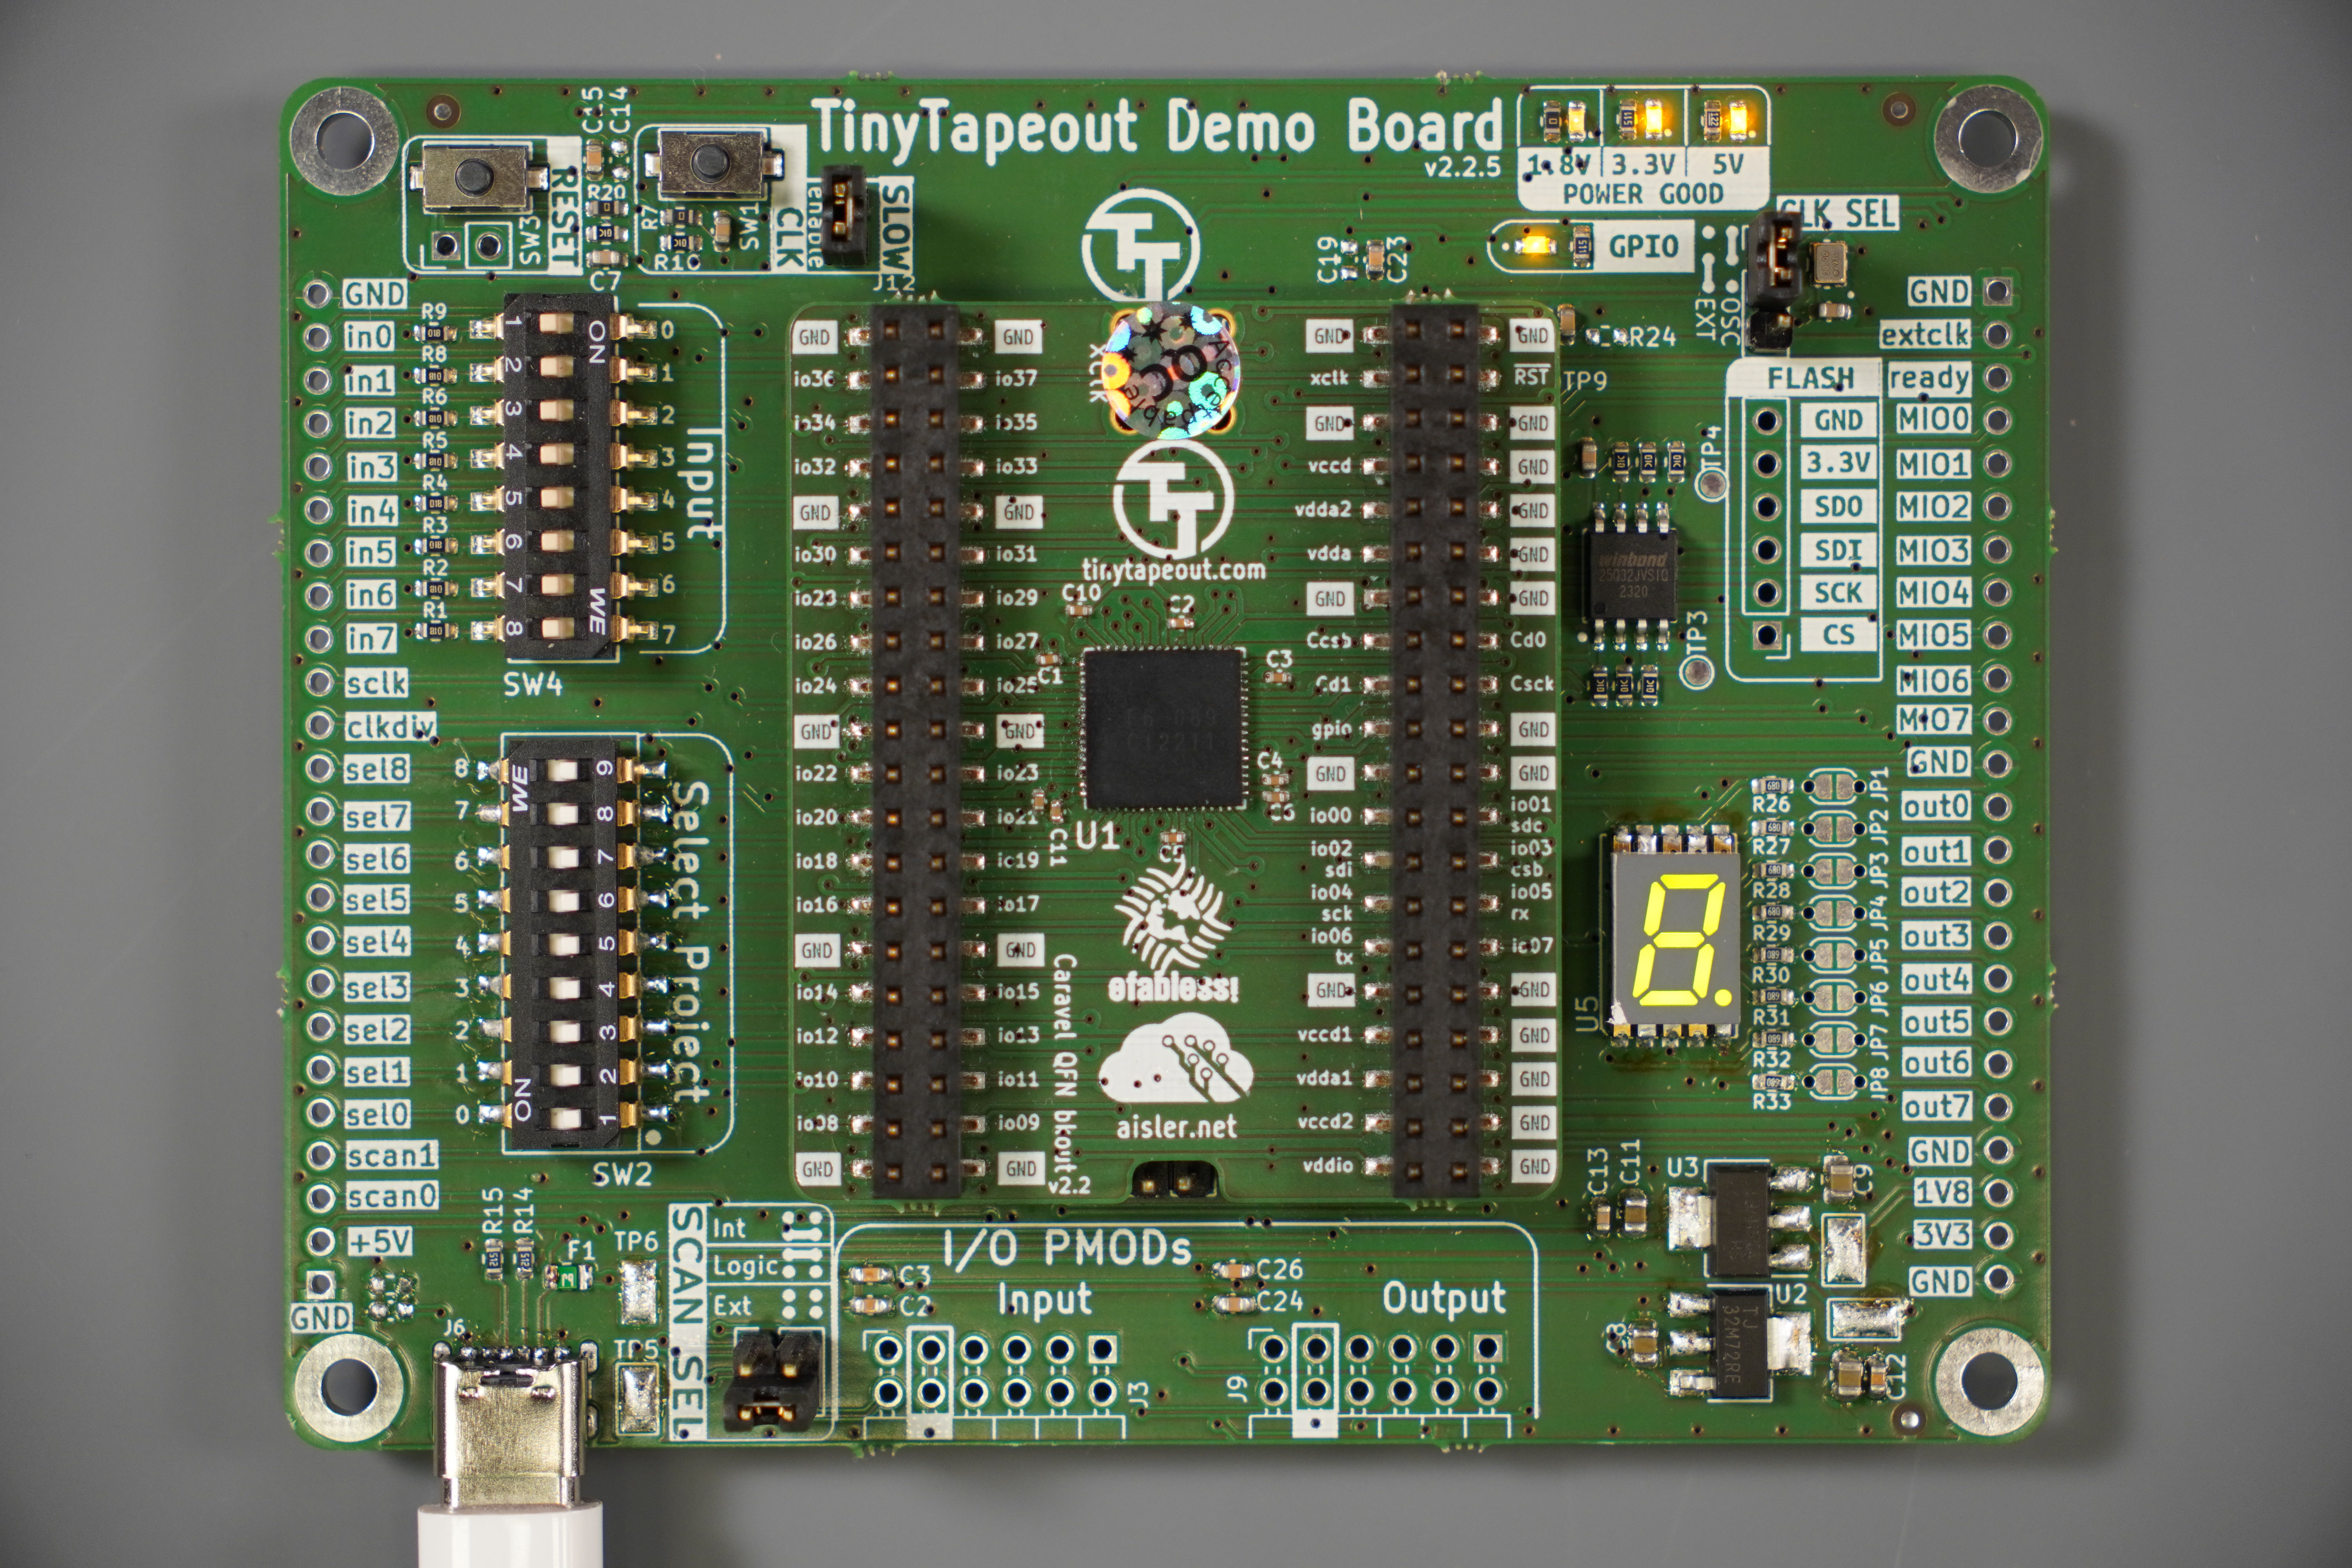
\includegraphics[width=0.5\textwidth]{./Figs/tt02 pcb assembled.JPG}
\caption{The demonstration board, which has been recorded as Certified Open Source Hardware ES000040~\cite{oshwacertification}.}
\label{fig:demonstration_board}
\end{figure}
